\chapter{Laser scanning~\cite{scanning-handbook}}

Jako Laser scanning se označuje technologie využívající rychle pohybující laserový paprsek, tento pohyb je často zprostředkovaný pohyblivými zrcátky.

Dle stylu pohybu zrcátek se technologie dají rozdělit na, polygonové skenery, galvanometrové skenery a MEMS skenery.

\section{Polygonové skenery}
Polygonové skenery se vyznačují rotujícím polygonem se zrcadlivými stranami. Při rotaci polygonu se mění úhel dopadu laserového paprsku na zrcátko, a díky tomu se mění směr odraženého paprsku, viz. \ref{fig:polygon-scanner}.

\begin{figure}[!htb]
  \centering
  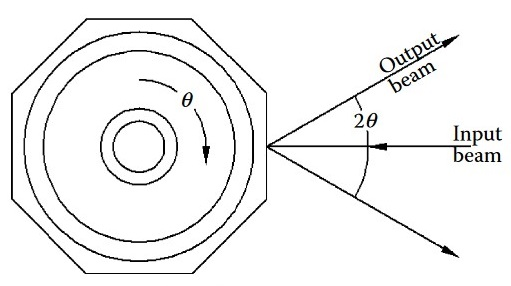
\includegraphics[width=0.5\textwidth]{img/polygon-scanner.jpg}
  \caption{\label{fig:polygon-scanner} mechanika polygonových skenerů}
\end{figure}

% \begin{figure}[!htb]
%   \centering
%   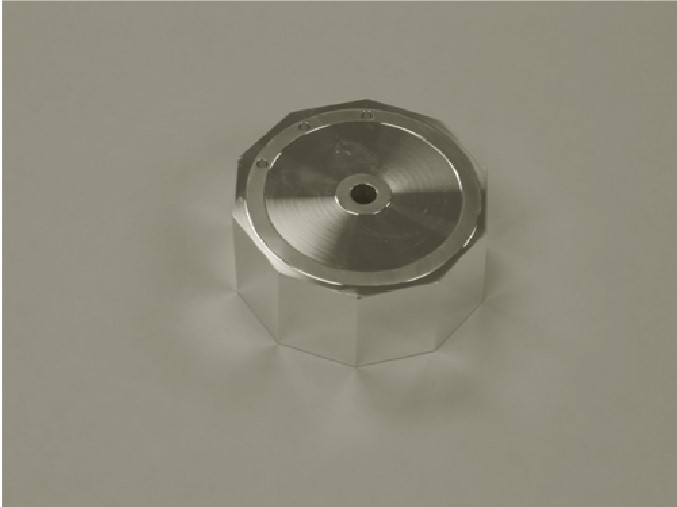
\includegraphics[width=0.5\textwidth]{img/polygon-prismatic-mirror.jpg}
%   \caption{\label{fig:polygon-prismatic-mirror} hranolové zrcátko polygonového skeneru}
% \end{figure}

% \begin{figure}[!htb]
%   \centering
%   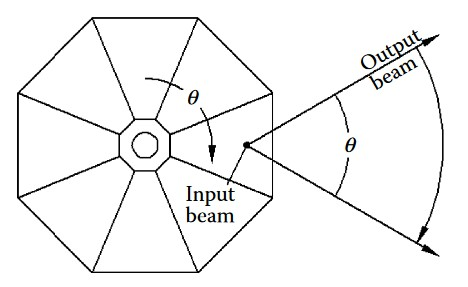
\includegraphics[width=0.5\textwidth]{img/polygon-pyramidal-mirror.jpg}
%   \caption{\label{fig:polygon-pyramidal-mirror} pyramidové zrcátko polygonového skeneru}
% \end{figure}
%

Pouze s jedním hranolem jsou polygonové skenery schopny směřovat paprsek pouze v jedné rovině - při projekci by bylo možné vykreslit maximálně přímku. Pokud je potřeba paprsek směřovat 

\begin{figure}[!htb]
  \centering
  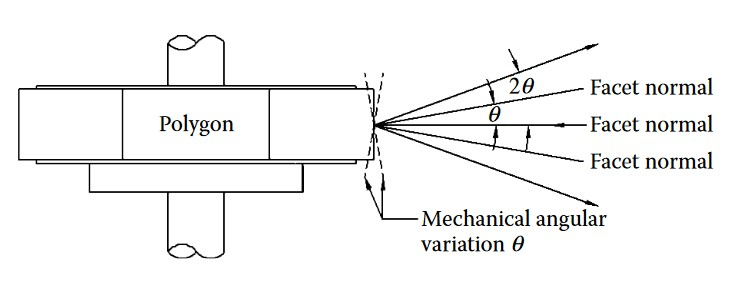
\includegraphics[width=0.8\textwidth]{img/polygon-angular-variation.jpg}
  \caption{\label{fig:polygon-angular-variation} úhlová rozdílnost polygonového skeneru}
\end{figure}


\begin{figure}[!htb]
  \centering
  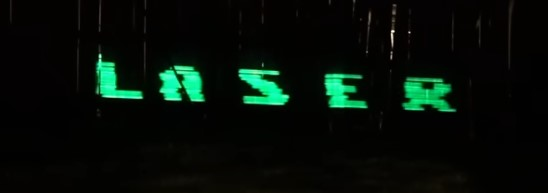
\includegraphics[width=0.5\textwidth]{img/harddrive-projection.jpg}
  \caption{\label{fig:harddrive-projection} příklad projekce laserového projektoru s polygonovým skenerem; zdroj \cite{harddrive-projector-youtube}}
\end{figure}

\section{Galvanometrové skenery}

ja vyuzivam galva, protoze se s nima da nejlip pohrat, jsou nejuniverzalnejsi a tim padem nejvic zaujmou - cil